\chapter{Storage of Materials}

\begin{multicols}{2}

\section{The Science Box}

\begin{center}
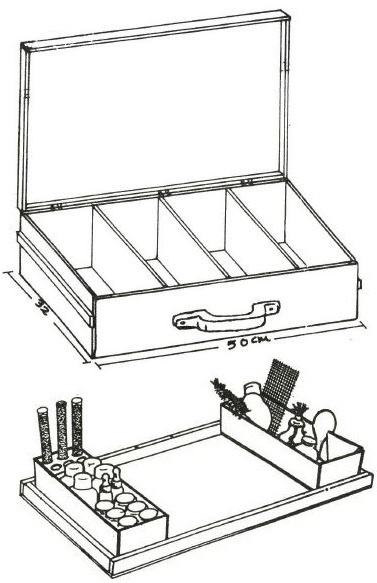
\includegraphics[width=0.33\textwidth]{./img/source/science-box-alt.jpg}
%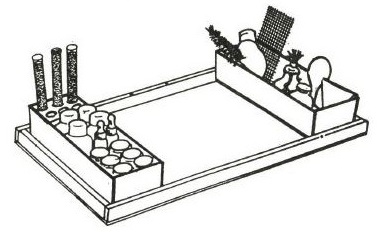
\includegraphics[width=0.35\textwidth]{./img/source/science-tray-alt.jpg}
\end{center}

\begin{itemize}
\item Use a metal storage trunk to organize all of your new, locally-made science equipment.
\item Metal or cardboard sheets can be used as dividers. Tape firmly in place.
\item Use the lid as a science tray for safely and easily moving liquids and chemicals.
\end{itemize}


\section{Card and Picture Boxes}

\begin{center}
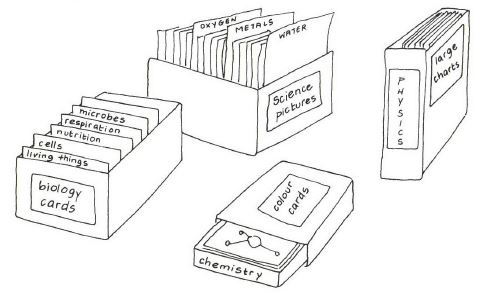
\includegraphics[width=0.49\textwidth]{./img/vso/card-boxes.jpg}
\end{center}

\begin{itemize}
%\item Select suitably-shaped boxes.
\item Cards and pictures can be stored
in all sorts of boxes. Store
according to syllabus topic or
alphabetically.
\item Dividers and compartments can
be made from cardboard.
\end{itemize}


\section{Matchbox Drawers}

\begin{center}
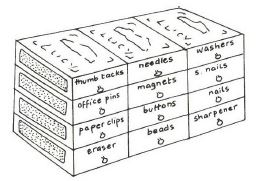
\includegraphics[width=0.3\textwidth]{./img/vso/matchbox-drawer.jpg}
\end{center}

\begin{itemize}
\item Drawers to store small items can
be made from matchboxes
glued together as shown.
\item Small pieces of string, wire or
buttons can be used as handles.
\end{itemize}


\section{Dividing Boxes}

\begin{center}
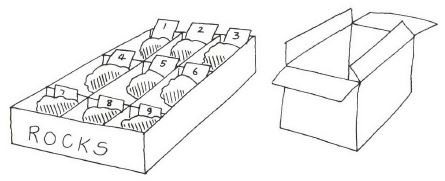
\includegraphics[width=0.45\textwidth]{./img/vso/dividing-boxes.jpg}
\end{center}

\begin{itemize}
\item Cut down the sides of boxes for
displays.
\item Samples can be sorted, then
displayed or stored in cardboard
boxes as shown.
\item The flaps from the top of the
box may be cut off and used as dividers for the same box.
\end{itemize}


\section{Envelopes and Bags}

\begin{center}
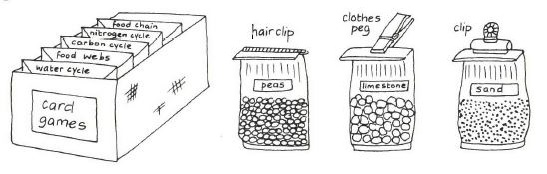
\includegraphics[width=0.49\textwidth]{./img/vso/envelopes-bags.jpg}
\end{center}

\begin{itemize}
\item Envelopes and bags of different
sizes can be used for storage.
Clearly label all containers.
\end{itemize}


%\section{Tins, Cups and Bottles}
%
%\begin{center}
%\includegraphics[width=0.49\textwidth]{./img/vso/tins-cups.jpg}
%\end{center}
%
%\begin{itemize}
%\item Tins, cups and bottles make good storage containers. Some items do
%not need lids, others do.
%\end{itemize}

\end{multicols}

%\section{Fold-Away Posters}
%
%\begin{center}
%\includegraphics[width=0.8\textwidth]{./img/vso/folding-posters.jpg}
%\end{center}
%
%\begin{itemize}
%\item Make your posters fold into the size of a book. It is easier if the
%poster is made from paper of the right size.
%\item After use, fold the poster along the original `book folds' and store in
%a cover.
%\end{itemize}

